Programmet kan køres via den udleverede .jar-fil. når programmet er startet op, skal man vælge hvilket data-sæt man vil benytte. BEMÆRK, nogle features er ikke fyldestgørende i OSM-datasættet.
Efter start af programmet kan det tage op til 5 sekunder før kortet ses på skærmen.

\begin{center}
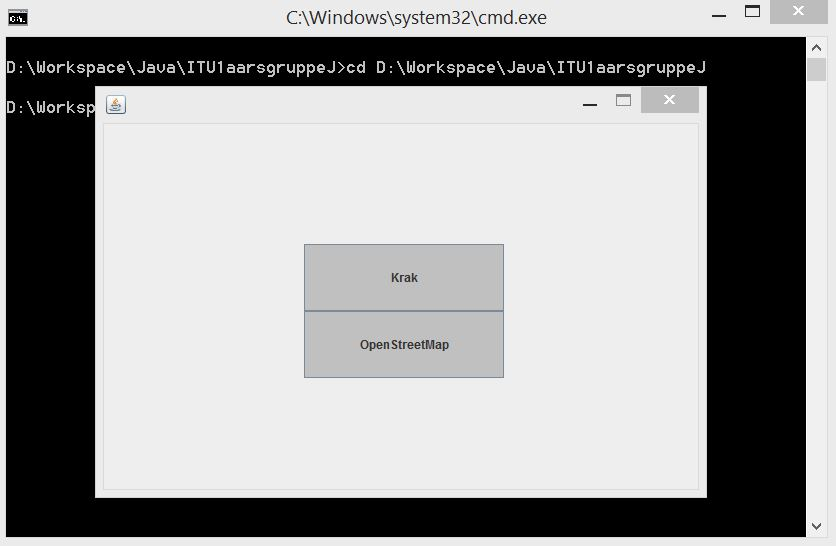
\includegraphics[width=(\textwidth)/2]{brugervejledning/vaelgdata}
\end{center}

\begin{center}
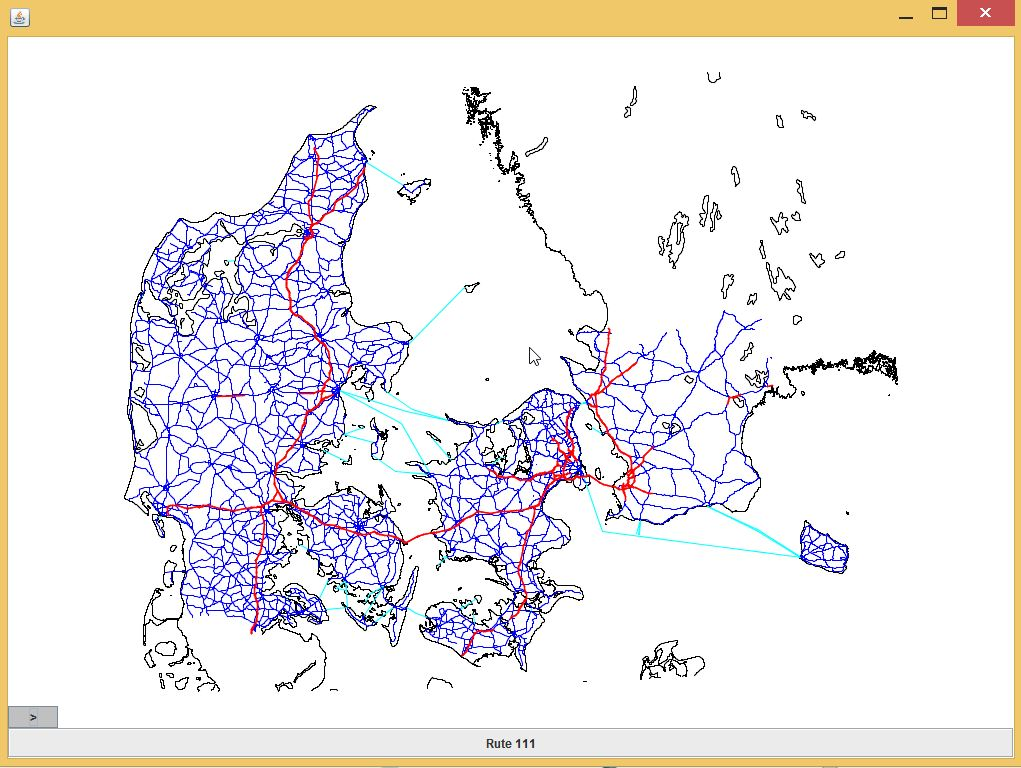
\includegraphics[width=(\textwidth)/2]{brugervejledning/renkort}
\end{center}

\subsection{kortmanipulation}
\begin{table}[h!t]
\centering
	\caption{Tastaturgenveje}
	\begin{tabular}{p{3cm} l l l}
		\hline\hline
		Kommando & Tast & Tast & Tast \\ [0.5ex]
		\hline
		Zoom kortet ind & i & + & num+\\
		Zoom kortet ud & o & - & num-\\
		Returner kortet til startzoomgrad og centrer kortet & r & backspace\\
		Bevæg kortet & piletasterne\\
		Vis/skjul rutevejledningsmenu & space \\
		\hline
	\end{tabular}
\end{table}

\begin{table}[h!t]
\centering
	\caption{Mussemanipulation}
	\begin{tabular}{p{3cm} l l p{5cm}}
		\hline\hline
		Kommando & bruger \\ [0.5ex]
		\hline
		Zoom kortet ind & Rul musehjulet væk fra bruger\\
		Zoom kortet ud & Rul musehjulet hen mod bruger\\
		Zoom kortet ind i markeret område & Højreklik, træk og slip så du har det ønskede udsnit\\
		Returner kortet til startzoomgrad og centrer kortet & Tryk på den midterste museknap\\
		Bevæg kortet & Venstreklik, træk og slip så du har det ønskede udsnit\\
		åbn/luk rutevejledningsmenu & benyt knappen nede i venstre hjørne\\
		\hline
	\end{tabular}
\end{table}

\subsection{rutevejledning}

Man kan enten  benytte musen på kortet for at få en rutevejledning, eller man kan benytte rutevejledningsmenuen. Man benytter musen ved at højreklikke på sin start posisiion, og så klikke med venstre mussetast på sin slutdestination. I tilfælde af at man benytte rutevejledningsmenuen, skriver man addressen på sin startdestination i felt (A) og sin slutdestination i felt (B), hvorefter man trykker på knappen: 'Get route'. Der vil nu vises en rutevejledning i rutevejledningsmenuen, såvel som at ruten vil være tegnet med en lyserød farve på kortet.

\begin{center}
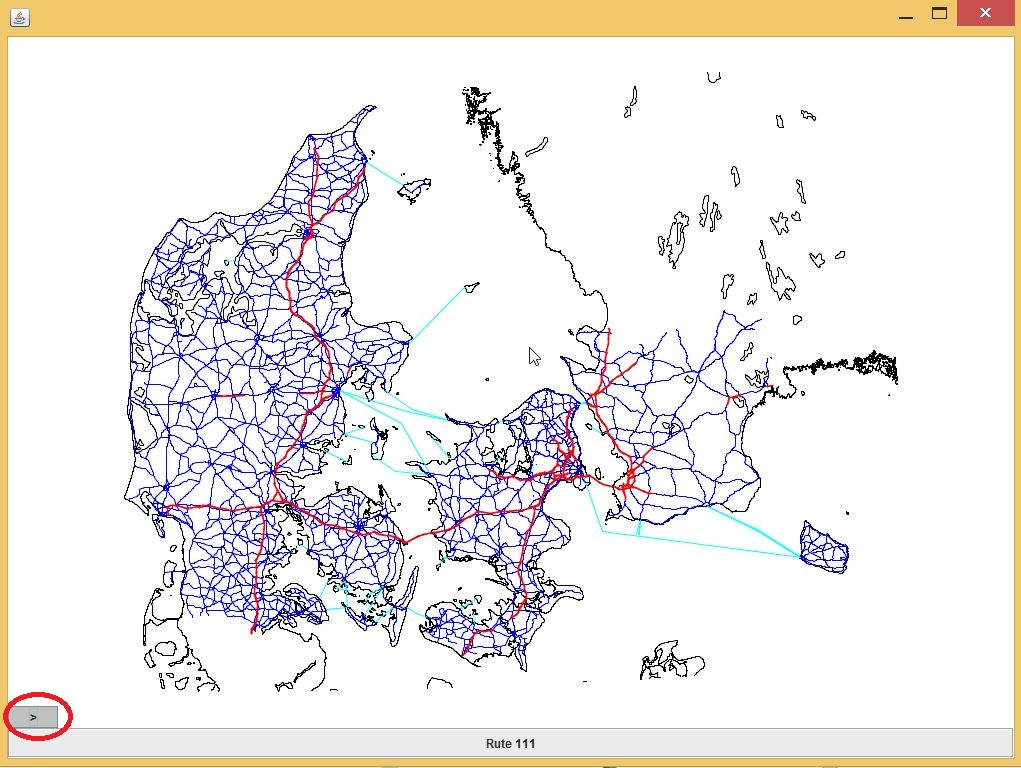
\includegraphics[width=(\textwidth)/2]{brugervejledning/halvrenkort}
\end{center}

\begin{center}
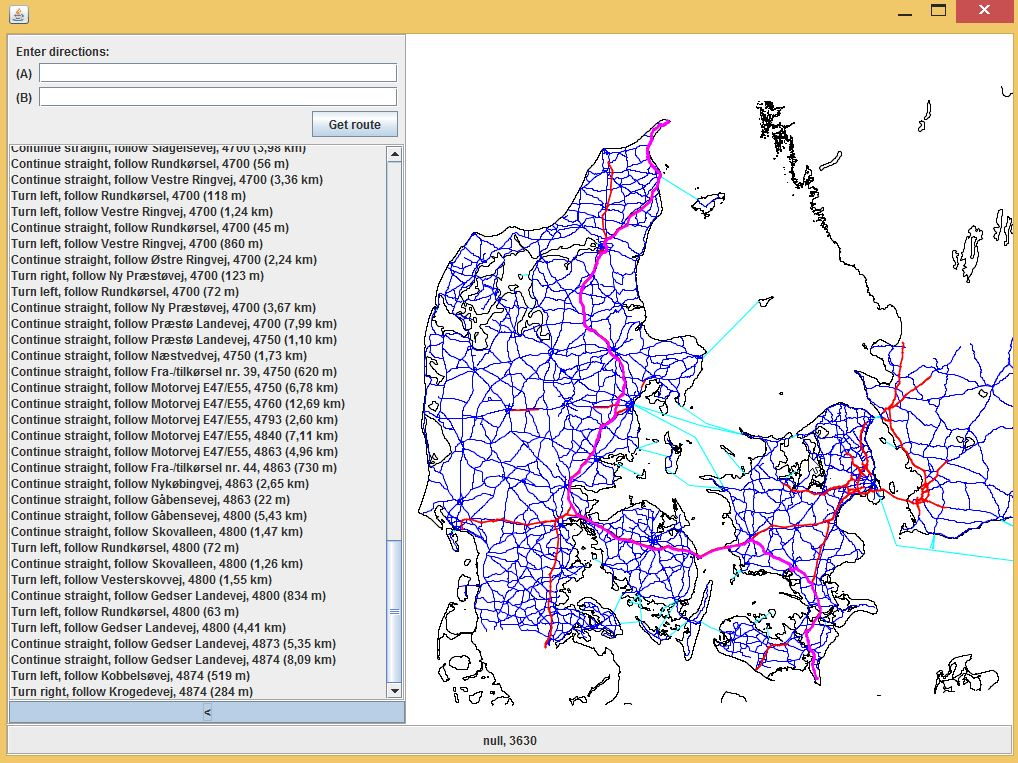
\includegraphics[width=(\textwidth)/2]{brugervejledning/klikkort}
\end{center}